\documentclass{beamer}
\beamertemplatenavigationsymbolsempty
\usecolortheme{beaver}
\setbeamertemplate{blocks}[rounded=true, shadow=true]
\setbeamertemplate{footline}[page number]
%
\usepackage[utf8]{inputenc}
\usepackage[english,russian]{babel}
\usepackage{amssymb,amsfonts,amsmath,mathtext}
\usepackage{subfig}
\usepackage[all]{xy} % xy package for diagrams
\usepackage{array}
\usepackage{multicol}% many columns in slide
\usepackage{hyperref}% urls
\usepackage{hhline}%tables
\usepackage{wrapfig}
% Your figures are here:
\graphicspath{ {fig/} {../fig/} }
\newtheorem{theorem_rus}{Теорема}
\newtheorem{lemma_rus}{Лемма}
\setbeamertemplate{theorems}[numbered]
%\setbeamertemplate{caption}[numbered]

%----------------------------------------------------------------------------------------------------------
\title[\hbox to 56mm{Мат. модель эффекта обратной связки с системах ИИ}]{Математическая модель эффекта обратной связи в системах искусственного интеллекта}
\author[А.\,С.~Веприков]{Андрей Сергеевич Веприков\\
\small Научный руководитель: д.ф.-м.н. А.\,С.~Хританков}
\institute{Кафедра интеллектуальных систем ФПМИ МФТИ\\
Специализация: Интеллектуальный анализ данных\\
Направление: 03.04.01 Прикладные математика и физика}
\date{2024}

%----------------------------------------------------------------------------------------------------------
\begin{document}
%----------------------------------------------------------------------------------------------------------
\begin{frame}
\thispagestyle{empty}
\maketitle
\end{frame}
%-----------------------------------------------------------------------------------------------------
\begin{frame}{Примеры процессов многократного машинного обучения}
    \begin{enumerate}
        %Иллюстрацией этого может быть модель прогнозирования цен на жилье, которая опирается на фактические покупки, рекомендованные моделью \cite{khritankov2021hidden}. Таким образом, модель частично учится на своих собственных прогнозах. Примеры подобных эффектов, таких как эхо-камеры и пузыри-фильтров, широко описаны в литературе \cite{michiels2022filter}. 

        \item Самоисполняющееся пророчество (self-fulfilling prophecy)
        
        \item Эффекты петель обратной связи (feedback loop) в рекомендательных системах \cite{khritankov2021hidden} 
        \item Дрейф данных (data drift) в системах предиктивного полицейского контроля \cite{ensign2018runaway}
        \item Усиление ошибок (error amplification) со временем в задаче медицинского прогнозирования \cite{adam2022error}
        % \item Пузыри фильтров (filter bubbles)
    \end{enumerate}
\end{frame}

\begin{frame}{Математическая модель эффекта обратной связи в системах искусственного интеллекта}
    \vspace{-2mm}
    В данной работе решается задача математического моделирования систем с адаптивным управлением. Системе с ИИ ставится в соответствие дискретная динамическая система, по поведению которой можно судить об исходном объекте.
    \vspace{-1mm}
    \begin{figure}
        \centering
        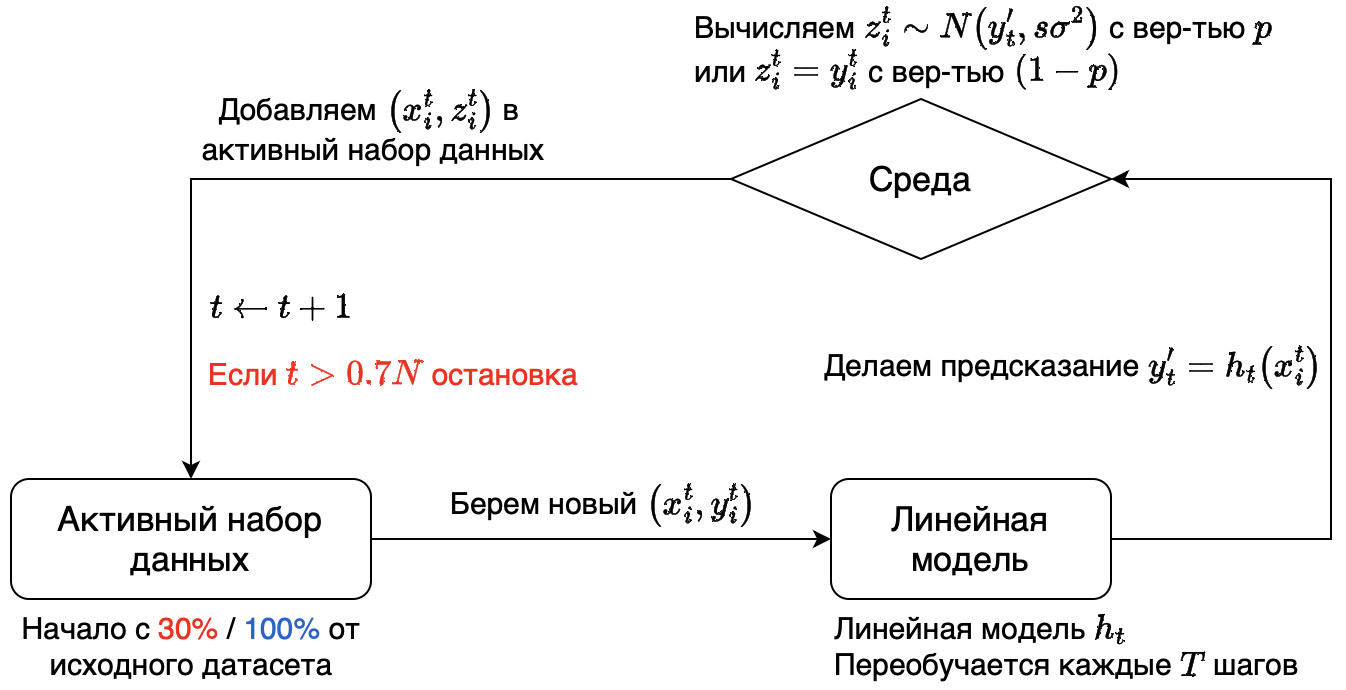
\includegraphics[width=0.85\textwidth]{fig/Experiment_setups.png}
        
        Две постановки эксперимента. \color{red}Скользящее окно \color{black}и \color{blue}обновление выборки.
        \label{exp}
    \end{figure}

\end{frame}

%----------------------------------------------------------------------------------------------------------
\begin{frame}{Постановка задачи и теорема о предельном множестве}
\vspace{-2mm}
 Определим дискретную динамическую систему:
    \begin{equation}
        \label{system}
        f_{t+1}(x) = \text{D}_t(f_t)(x) ~ \text{ для } ~ \forall x \in \mathbb{R}^n, t \in \mathbb{N} ~\text{ и } ~ \text{D}_t \in \mathbb{D},
    \end{equation}
    где $\text{D}_t$ -- оператор эволюции, $x$ -- вектор данных в моделируемой системе, $f_t(x)$ -- функции плотности.  
    %\begin{columns}[c]
    %\column{0.7\textwidth}
    \begin{theorem_rus}[Веприков, 2023. Предельное множество системы \eqref{system}] \label{delta}
        \begin{wrapfigure}[7]{r}{0.45\textwidth}
        \vspace{-0.61cm}
        \hspace{-6mm}
        \begin{minipage}{0.45\textwidth}
        \vspace{-0.57cm}
        \begin{figure}
        %\centering
        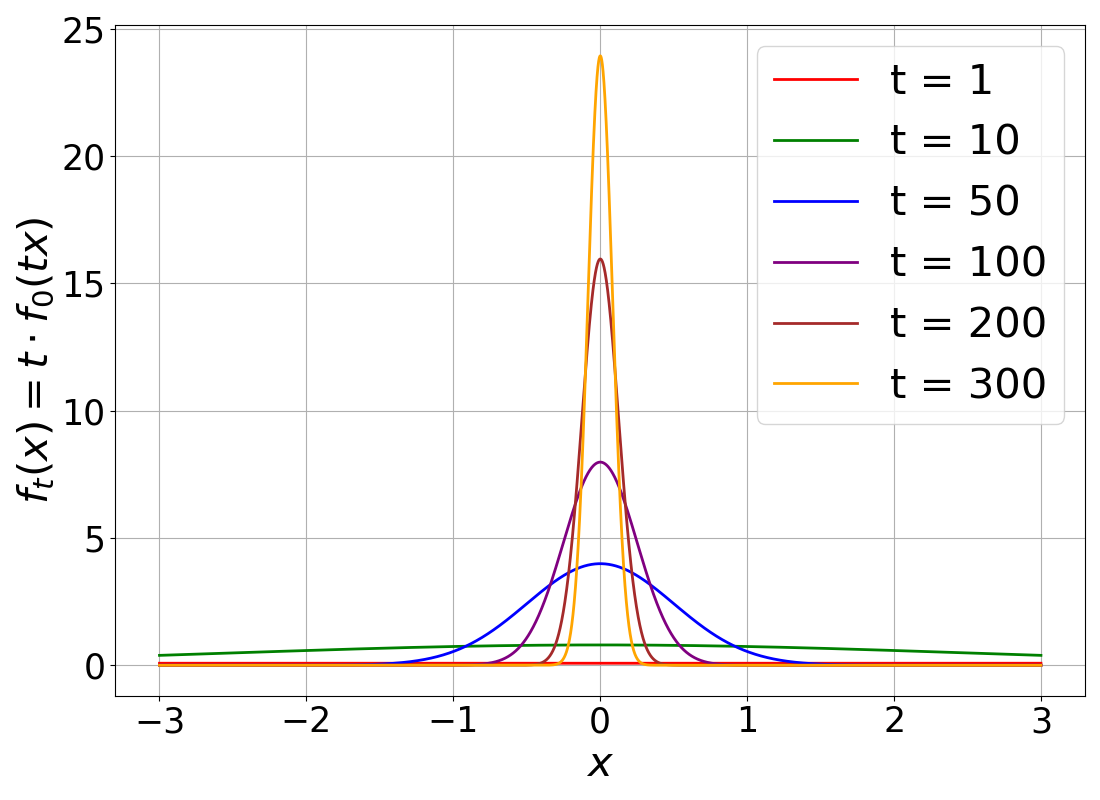
\includegraphics[width=1.22\textwidth]{fig/fig1_Normal.png}
    
        %\footnotesize{Пример использования Теоремы \ref{delta} с $\psi_t = t$ для $\mathcal{N}(0; 1)$.}
        \end{figure}
        \end{minipage}
    \end{wrapfigure}
        Для любой функции плотности $f_0$ и дискретной динамической системы \eqref{system}, пусть существуют $ g \in L_1\left(\mathbb{R}^n\right)$ и $\psi_t \geq 0$ такие, что \color{blue}$f_t\left(x\right) \leq \psi_t^n \cdot |g(\psi_t \cdot x)|$. %для всех $t \in \mathbb{N}$ и $x \in \mathbb{R}^n$.
    
        \color{black}Тогда, если $\psi_t \to \infty$, плотности $f_t(x)$ стремятся к дельта-функции, $f_t(x) \underset{t \to +\infty}{\longrightarrow} \delta(x)$ слабо.  
    
        Если $\psi_t \to 0$, тогда плотности $f_t(x)$ сходятся к нулевому распределению, $f_t(x) \underset{t \to +\infty}{\longrightarrow} \zeta(x)$ слабо.
    \end{theorem_rus}
    %\column{0.4\textwidth}
    %\end{columns}
\end{frame}
%----------------------------------------------------------------------------------------------------------
\begin{frame}{Анализ условий существования петель обратной связи}
    \vspace{-1mm} 
    Для задачи регрессии, когда данные имеют вид $\{(\textbf{x}^i, \textbf{y}^i) \}_{i=1}^N$ Теорема \ref{delta} записывается не для данных в системе ИИ, а для случайного вектора невязок модели $h$, вида $\textbf{y} - h(\textbf{x})$.
    \vspace{-1mm}
    \begin{lemma_rus}[Веприков, 2023. Стремление моментов к нулю] \label{moments}
        Если система \eqref{system} с $n=1$ удовлетворяет условиям Теоремы~\ref{delta} и $\psi_t \to \infty$, тогда все $2k$-тые моменты невязок 
        $\textbf{y} - h(\textbf{x})$ убывают со скоростью как минимум $\psi_t^{-2k}$.
    \end{lemma_rus}
    \vspace{-2mm}
    \begin{figure}
        \centering
        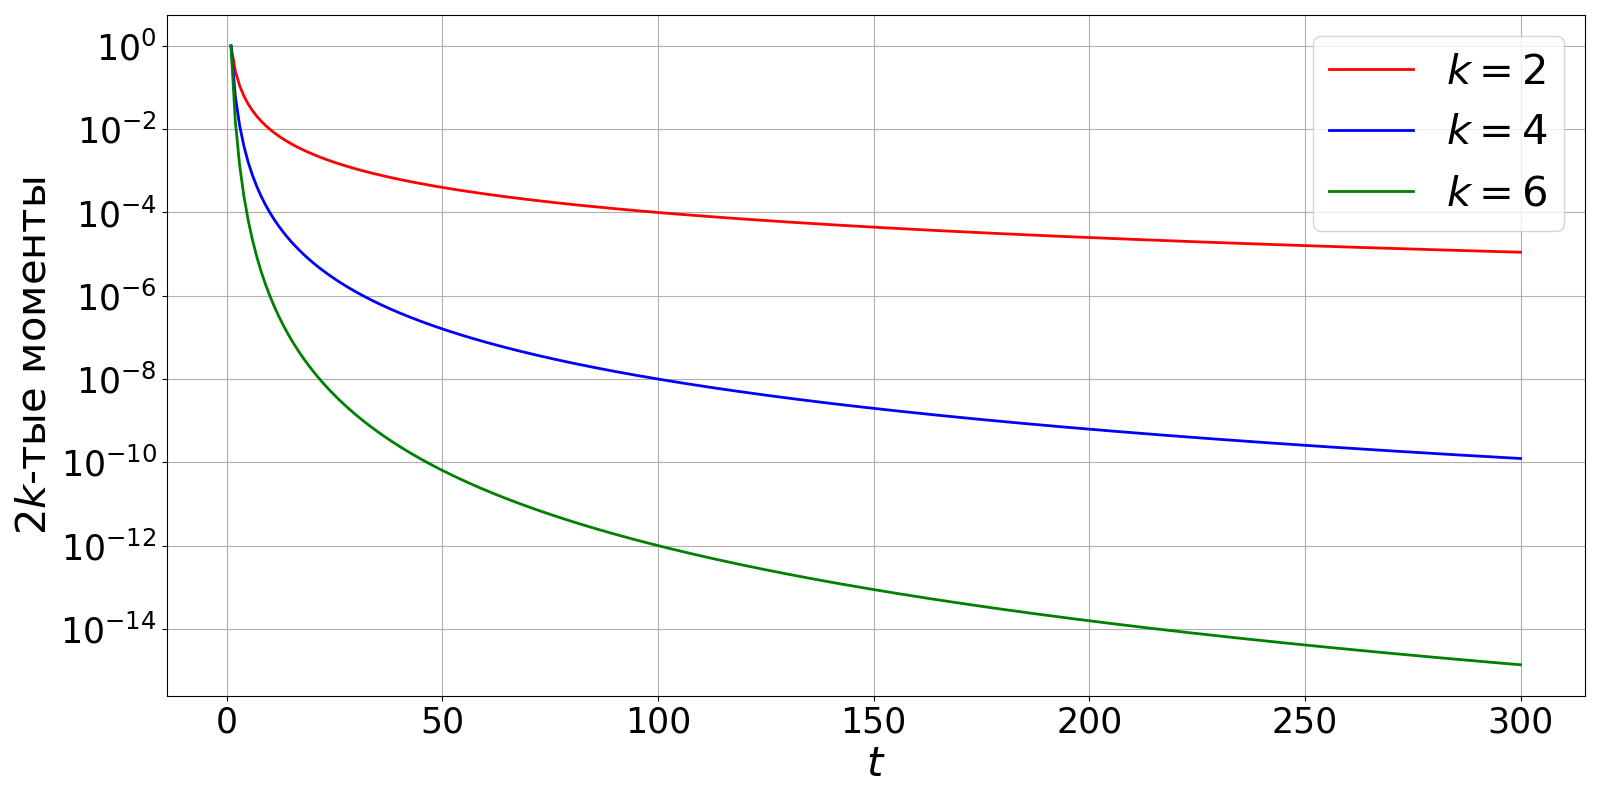
\includegraphics[width=0.85\textwidth]{fig/fig2.png}
        \vspace{-3mm}
        
        Пример использования Леммы \ref{moments}.
    \end{figure}
\end{frame}
\begin{frame}{Анализ автономности системы \eqref{system}}
    \begin{theorem_rus}[Веприков, 2023. Критерий автономности] \label{semigroup}
        Если операторы эволюции $\text{D}_t$ динамической системы \eqref{system} имеют вид $\text{D}_{\overline{1, t}}(f_0)(x) = \psi_t^n \cdot f_0(\psi_t \cdot x)$, тогда система \eqref{system} автономна тогда и только когда, когда \color{blue}
        $
            \psi_{\tau + \kappa} = \psi_{\tau} \cdot \psi_{\kappa} ~\forall \tau, \kappa \in \mathbb{N}.
        $
        \color{black}
    \end{theorem_rus}

    \begin{figure}
        \centering
        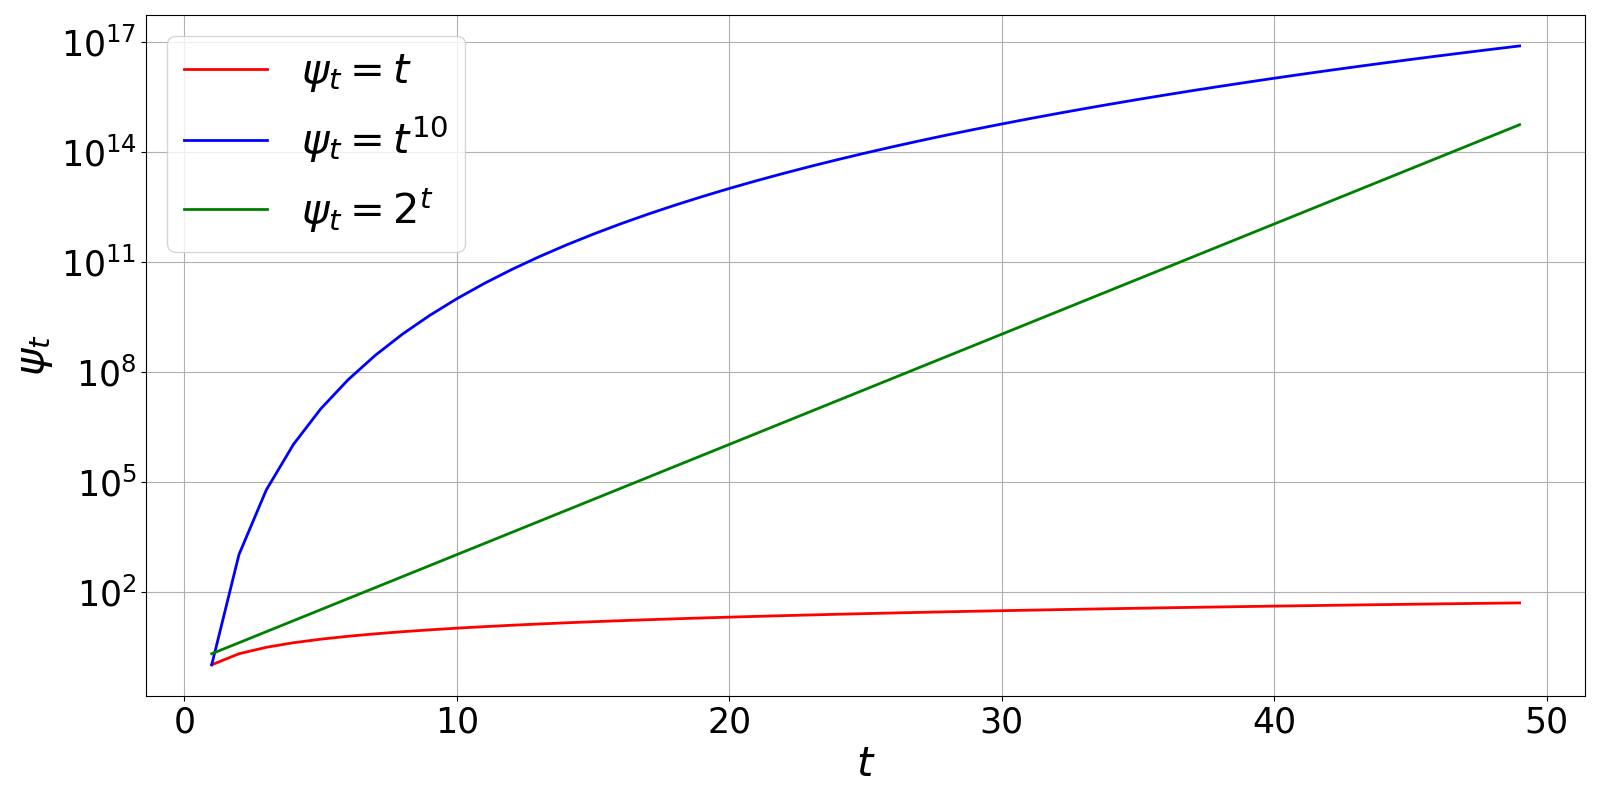
\includegraphics[width=0.95\textwidth]{fig/fig3.png}

        Пример использования Теоремы \ref{semigroup}.
    \end{figure}
\end{frame}
%----------------------------------------------------------------------------------------------------------
\begin{frame}{Предел к дельта-функции или нулевому распределению}
        \begin{figure}
            \centering
            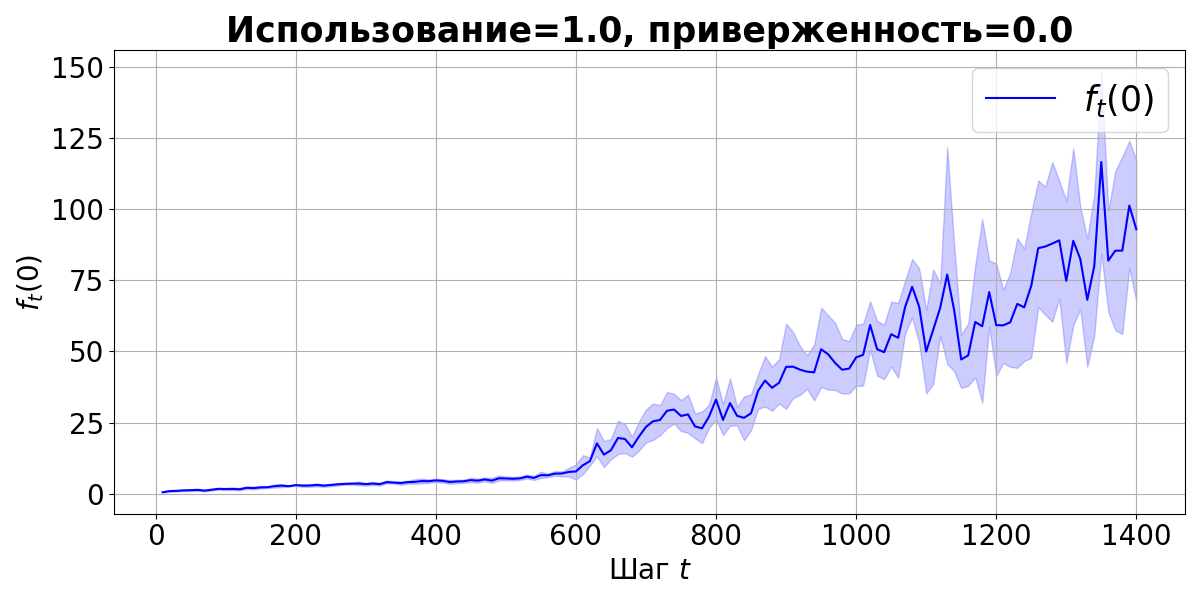
\includegraphics[width=0.5\textwidth]{fig/ft0_sw_synthetic_sgd_model_50_1.0_0.0.png}~
            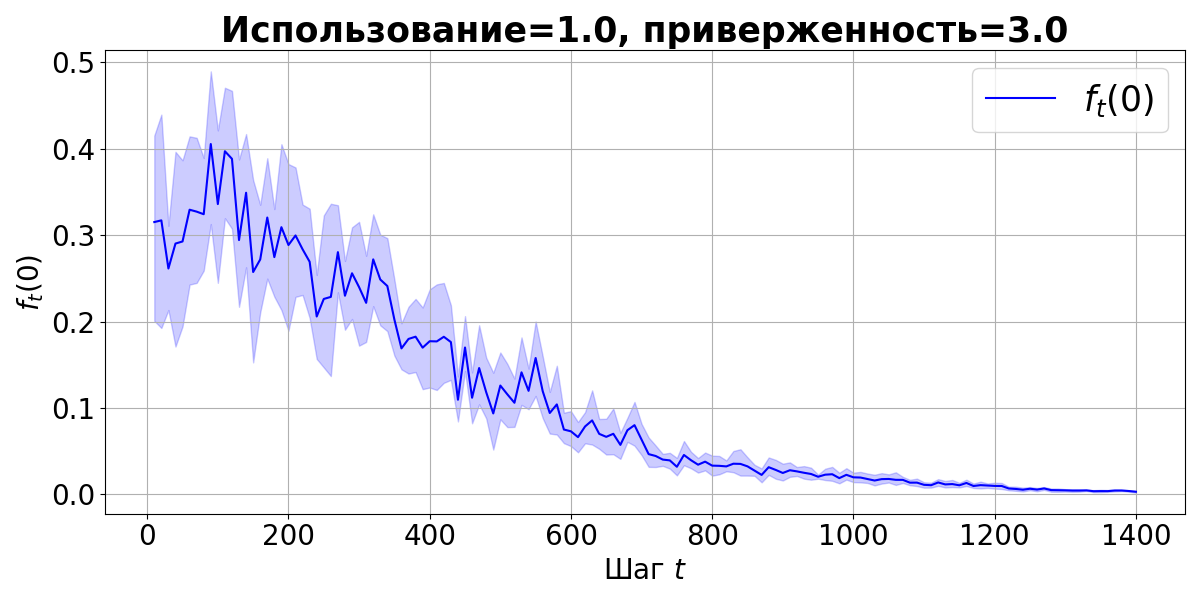
\includegraphics[width=0.5\textwidth]{fig/ft0_sw_synthetic_sgd_model_50_1.0_3.0.png}

            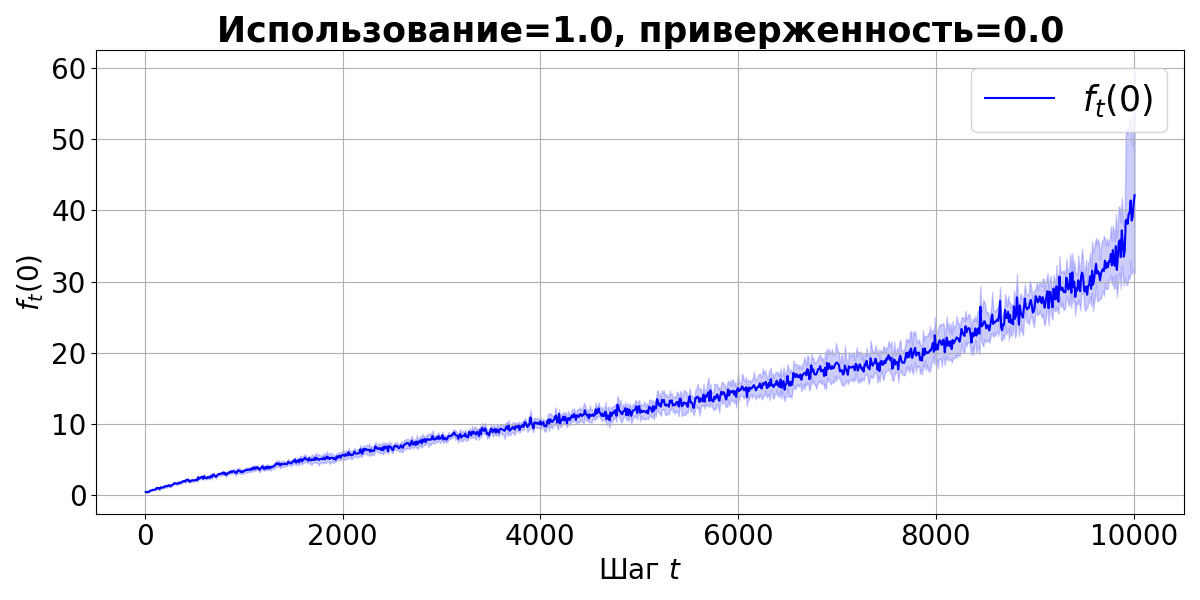
\includegraphics[width=0.5\textwidth]{fig/ft0_su_synthetic_sgd_model_50_1.0_0.0.png}~
            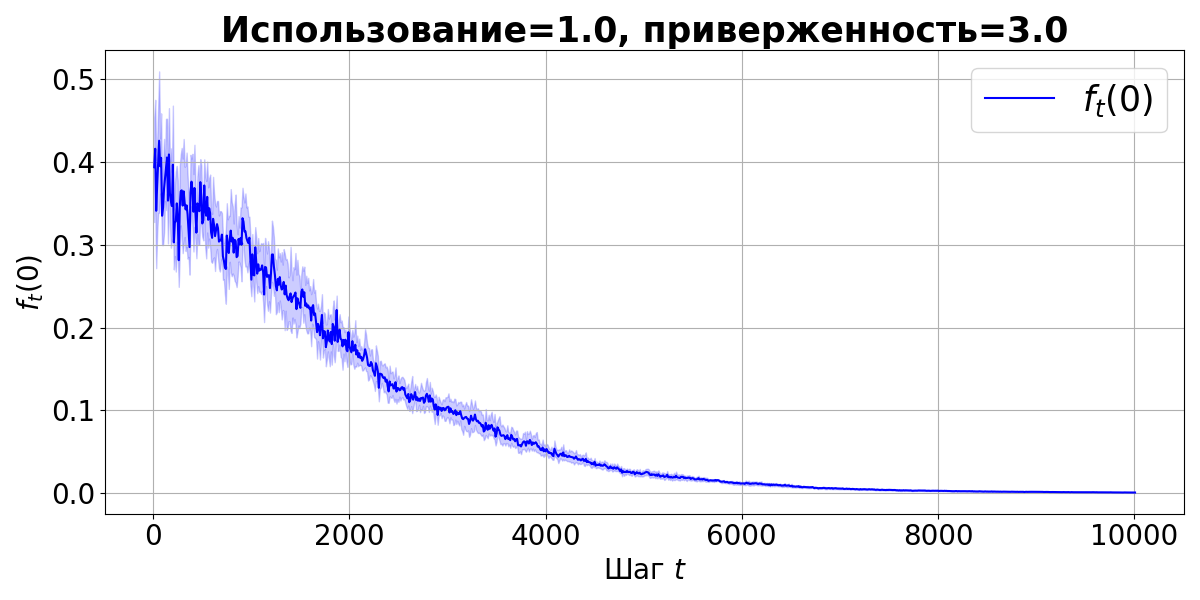
\includegraphics[width=0.5\textwidth]{fig/ft0_su_synthetic_sgd_model_50_1.0_3.0.png}
    
            Постановка скользящее окно (сверху), обновление выборки (снизу).
        \end{figure}
    \end{frame}

    \begin{frame}{Стремление моментов к нулю}
        \begin{figure}
            \centering
            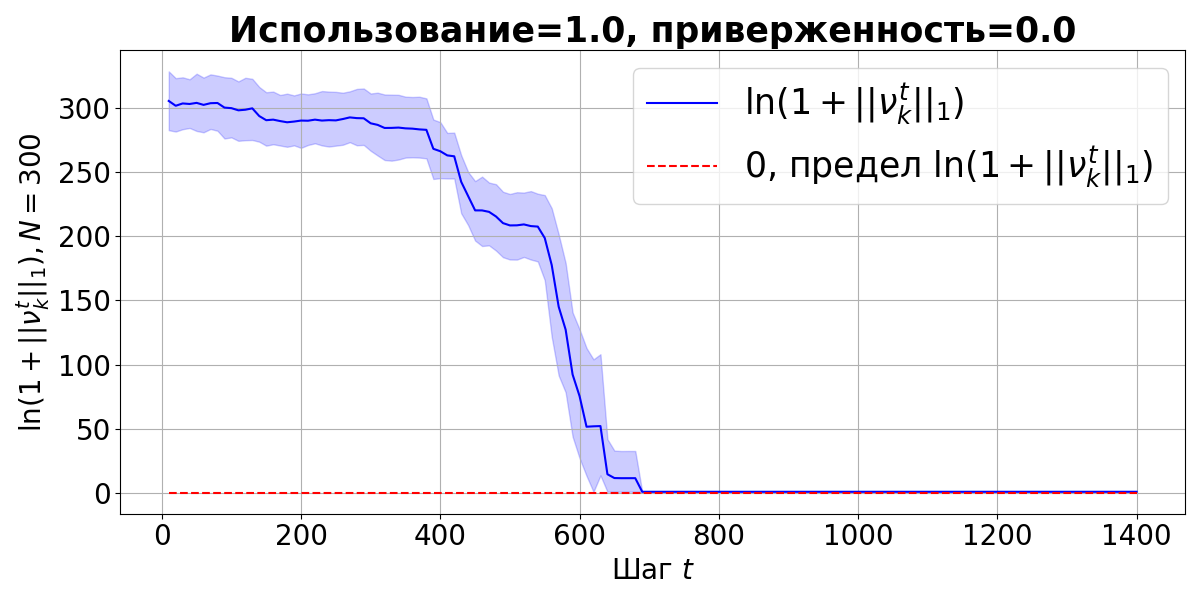
\includegraphics[width=0.65\textwidth]{fig/k_mom_sw_synthetic_sgd_model_50_1.0_0.0.png}~

            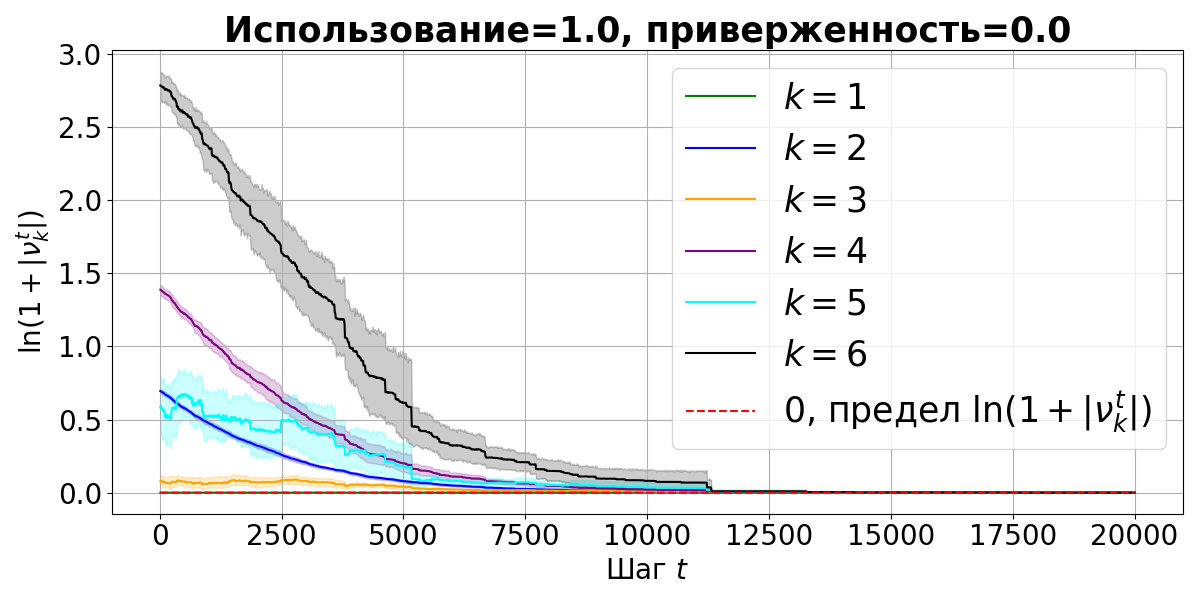
\includegraphics[width=0.65\textwidth]{fig/k_mom_su_synthetic_sgd_model_50_1.0_0.0.png}

            Постановка скользящее окно (сверху), обновление выборки (снизу).
        \end{figure}
    \end{frame}

    \begin{frame}{Исследование систем на автономность}
        \begin{figure}
            \centering
            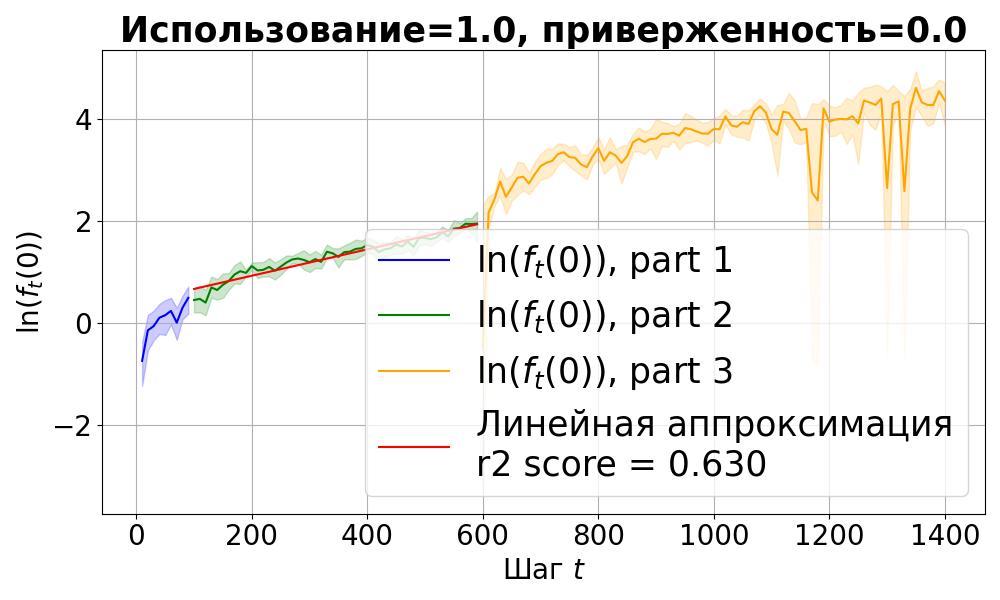
\includegraphics[width=0.51\textwidth]{fig/aut_sw_synthetic_sgd_model_50_1.0_0.0.png}
            
            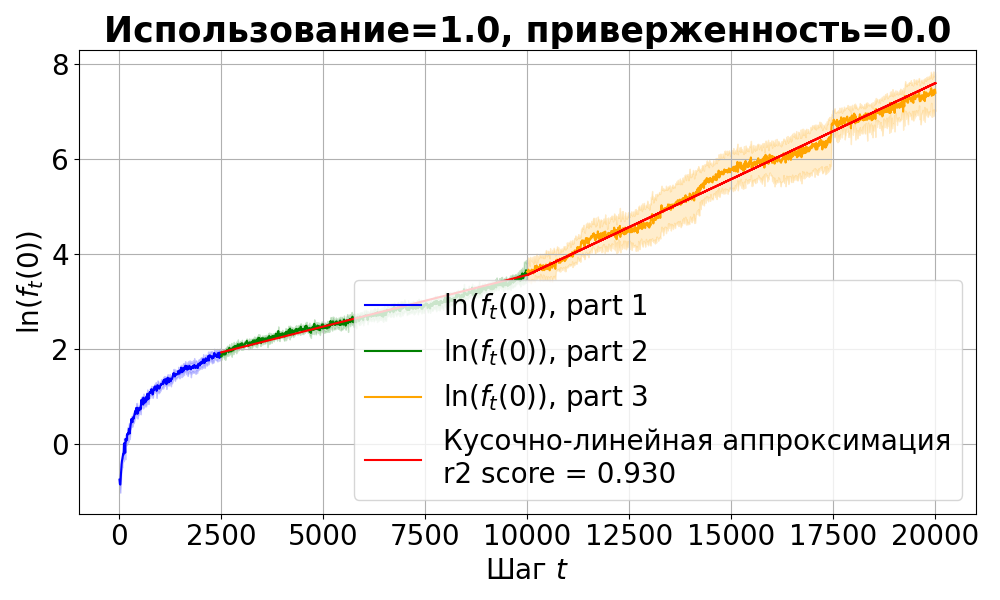
\includegraphics[width=0.49\textwidth]{fig/aut_su_synthetic_sgd_model_50_1.0_0.0.png}
            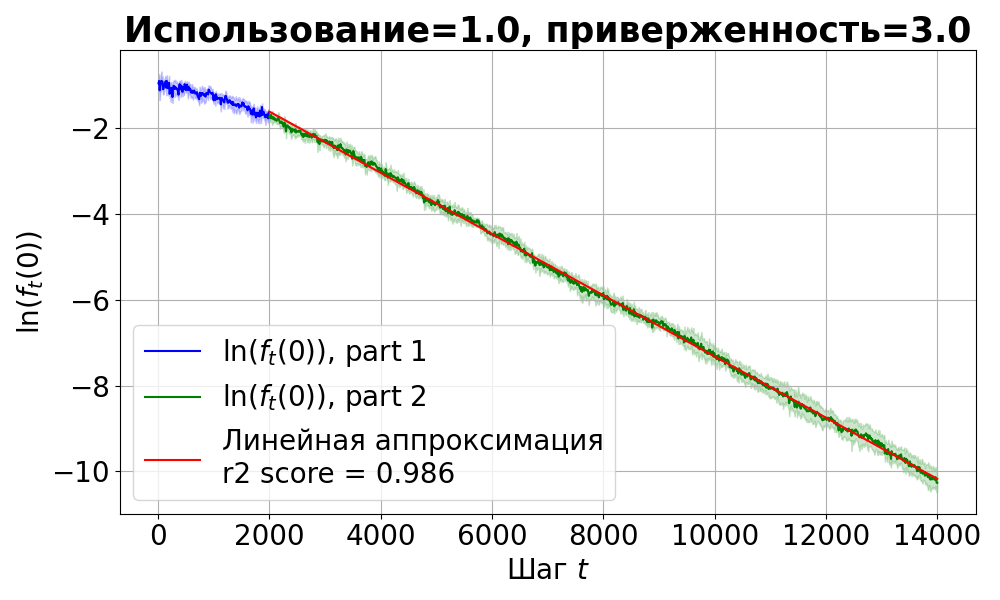
\includegraphics[width=0.49\textwidth]{fig/aut_su_synthetic_sgd_model_50_1.0_3.0.png}

            Постановка скользящее окно (сверху), обновление выборки(снизу).
        \end{figure}
    \end{frame}
%----------------------------------------------------------------------------------------------------------
\begin{frame}{Выносится на защиту}
    \begin{enumerate}
        \item Построена математическая модель эффекта петель обратной связи с использованием дискретных динамических систем
        \item Были получены результаты для определения предельного множества динамической системы, достаточных условий существования петли обратной связи и критерий автономности
        \item Разработан стенд проведения вычислительных экспериментов, симулирующий процесс многократного машинного обучения
    \end{enumerate}
\end{frame}
\begin{frame}{Публикации}
    \begin{enumerate}
        \item Подана статья в Q1 журнал <<Journal of Machine Learning Research>> (JMLR). Preprint: Veprikov A.,   Afanasiev A., Khritankov A. A Mathematical Model of the Hidden Feedback Loop Effect in Machine Learning Systems // arXiv preprint \url{https://arxiv.org/abs/2405.02726}

        \item Веприков А. С., Афанасьев А. П., Хританков А.С. Математическая модель эффекта обратной связи в системах искусственного интеллекта // Сборник тезисов 21-й Всероссийской конференции Математические методы распознавания образов (ММРО-21). – Российская академия наук, 2023. – С. 35-37 

        \item Подана статья в журнал <<Искусственный интеллект и принятие решений>> (ИИПР)
    \end{enumerate}
\end{frame}
\begin{frame}{Список литературы}
    \footnotesize
    \bibliographystyle{apalike}
    \bibliography{refs}
\end{frame}
%----------------------------------------------------------------------------------------------------------
\end{document} 